\documentclass[9pt]{beamer}
\usepackage{styles/mypreamble}
%~~~~~~~~~~~~~~~~~~~~~~~~~~~~~~~~~~~~~~~~~~~~~~~~~~~~~~~~~~~~~~~~~~~~~~~~~~~~~~
\title{Алгоритмы машинного обучения}
\subtitle{Лекция 10. Переобучение, регуляризация. Ridge, Lasso.}
\author{Владимир Кукушкин}
\institute{СПбГЭУ - 2020}
\date{\today}
%~~~~~~~~~~~~~~~~~~~~~~~~~~~~~~~~~~~~~~~~~~~~~~~~~~~~~~~~~~~~~~~~~~~~~~~~~~~~~~

\begin{document}

\titlepage

\section{Что такое переобучение}
\subsection{Описание явления переобучения}

\begin{frame}{Пример}
\begin{itemize}
    \item Решаем задачу интерполяции многочленами. Степень многочлена $n$ -- параметр семейства моделей. Минимизируем MSE.
    \item Казалось бы, с увеличением степени многочлена мы делаем MSE всё меньше и меньше,
    \item Однако несмотря на почти идеальное приближение существующих точек, очевидно что для другой выборки точек данной функции MSE будет очень большой.
    \item Таким образом, более сложная модель слишком сильно подстроилась под имеющиеся данные, потеряла \textit{способность к обобщению} и стала непригодной для практического использования. Такое явление называется \textbf{перебоучением} (a.k.a. overfitting).
\end{itemize}
\begin{center}
    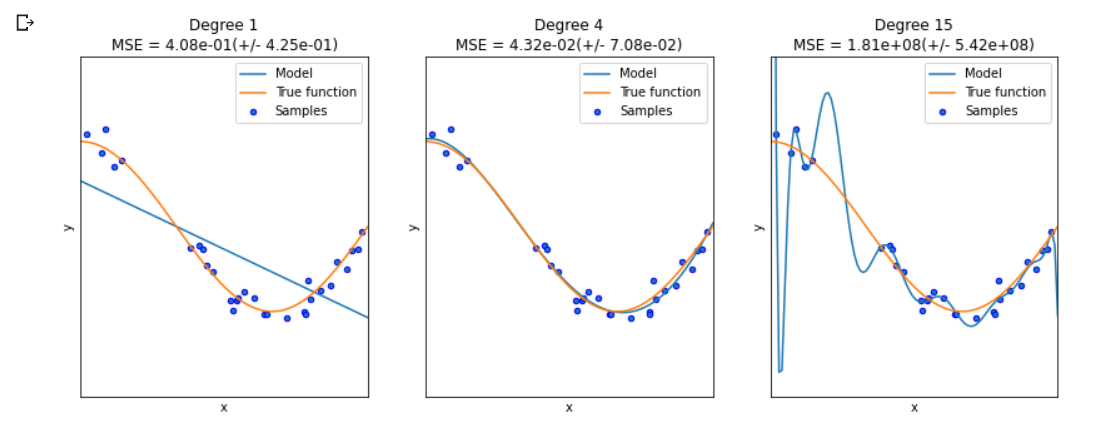
\includegraphics[height=0.35\textheight]{img/underfitting_overfitting.png}
\end{center}
\end{frame}

\begin{frame}{Формализация проблемы}
    \begin{itemize}
        \item Почему так происходит?
        \item Пусть у нас есть датасет $\mathcal{T}$. Тогда при обучении мы минимизируем ошибку $L(a, \mathcal{T})$. На самом же деле мы хотим минимизировать $Err = E(L(a, \mathcal{T}))$ по всем множествам $\mathcal{T}$.
    \end{itemize}
Борьбе с переобучением в ML -- это очень важно!
\end{frame}

\begin{frame}{Train, validation, test}
    \begin{itemize}
        \item Раз мы поняли, что минимизируя ошибку на данных обучения, у нас нет гарантии на минимизацию $Err$, давайте обучаться на одних данных, а проверяться на других.
        \item Разбиваем по объектам: $X = X_{train} \sqcup X_{test}$. На $X_{train}$ обучаемся, на $X_{test}$ замеряем качество модели. 
        \item Обычно в технологическом ML-процессе мы проверяем много моделей из разных семейств. По идее, после подбора оптимальных параметров для каждого семейства, нам надо посмотреть на качество модели на $X_{test}$ и принять решение, какая из них лучше. Но это также ведёт к переобучению: имея доступный $X_{test}$ мы будем неявно подглядывать в него, и выбирать ту модель, которая на нём покажет лучший результат.
        \item $X = X_{train} \sqcup X_{validation} \sqcup X_{test}$. На $X_{train}$ обучаемся, на $X_{validation}$ выбираем лучшую модель из семейства, на $X_{test}$ выбираем лучшую модель из всех. В идеале, $X_{test}$ должен быть скрытым и применяться только один раз.
        \item Доли разбиения -- на ваше усмотрение. Hastie пишет о 50\%-25\%-25\%.
    \end{itemize}
\end{frame}

\begin{frame}{Проблема}
\begin{itemize}
    \item Что если нам повезло с разбиением, и попались халявные validation/test? Измерение ошибки по-прежнему смещено в сторону конкретных validation/test, и пока об обобщении $Err$ речи не идёт.
    \item Если бы у нас был доступ ко всей генеральной совокупности данных, то мы бы набрали бы много тестов, и установили $Err$ как среднюю ошибку.
    \item Но как правило, у нас есть доступ только к одному датасету $X$.
\end{itemize}
\end{frame}

\subsection{Кросс-валидация}

\begin{frame}{Кросс-валидация (K-fold cross-validation)}
\begin{itemize}
    \item Будем считать, что тест у нас отделён, и отделять его от $X$ не нужно. Разобьём $X$ на $K$ примерно равных частей. Построим K разбиений вида $X = X_{-i} \sqcup X_{i}$, $i=1,\ldots, K$, где $X_{i}$ -- одна из $K$ частей (validation), а $X_{-i}$ -- всё остальное (train).
    \item Выбираем лучшую модель по средней ошибке, показанной на всех $K$ валидейтах:
    $$CV(a, X) = \frac{1}{K} \sum_{i=1}^K L(\hat a(X_{t_i}), X_{v_i}).$$
    \item Таким образом, каждый элемент данных имеет возможность поучаствовать в замере качества. Такая оценка $Err$ уже будет несмещённой (при условии, что $X$ репрезентативен).
    \item На практике $K$ выбирают от нескольких единиц до нескольких сотен. В зависимости от объёмов и рисков получить смещение.
\end{itemize}
\includegraphicsheight{0.2}{img/cross_validation.png}
\end{frame}

\begin{frame}{Leave-one-out}
    \begin{itemize}
        \item Предельный случай: $K$ = $N$. То есть Обучаемся на всех эдементах без одного, проверяемся на одном.
        \item Оценка получается также несмещённой и более точной.
        \item Однако это слишком ресурсоёмко. Нужно $N$ раз обучать модели.
        \item Поэтому на практике для больших датасетов ограничиваются $K$ порядка нескольких сотен.
    \end{itemize}
\end{frame}

\subsection{Bias VS Variance}
\begin{frame}{Декомпозиция ошибки}
    \begin{itemize}
        \item Предположим, что существует точная зависимость $y = f(x) +\varepsilon$, где $\varepsilon$ случайный шум с параметрами $\mathcal{E}\varepsilon = 0$ и $D\varepsilon = \sigma^2_\varepsilon$.
        Тогда верно разложение
        $$Err = E[(y - \hat a(x))^2] = \sigma^2_\varepsilon + (\underbrace{E\hat a(x) - f(x)}_{Bias})^2 + \underbrace{E(\hat a(x) - E\hat a(x))^2}_{Variance}.$$
        \item То есть ожидание квадрата ошибки состоит из неустраняемой дисперсии шума, смещения предсказания относительно правильного (bias) и разброса предсказания (variance).
    \end{itemize}
\end{frame}

\framedgraphic{Иллюстрация}{img/bias_variance.png}

\begin{frame}{Симуляция}
\begin{itemize}
    \item Посмотрим, как зависит качество предсказание от сложности модели в контексте bias и variance.
    \item Модель -- линейная регрессия (точнее, lasso. об этой модели поговорим позже). Сложность модели будем регулировать количеством фич.
    \item Сгенерируем 100 датасетов, обучимся на каждом и замерим ошибку трейне и валидейте.
    \item Видим (см. следующий слайд), что при повышении сложности модели на трейне увеличивается точность и уменьшается дисперсия: модель получает возможность уловить мельчайшие различия.
    \item Однако на тесте при этом, начиная с некоторого момента, перестаёт расти точность и даже начинает немного падать, а вот дисперсия начинает расти очень сильно. Именно это и свидетельствует о переобучении: на разных тестах наша модель будет вести себя непредсказуемо.
    \item Вывод: крайности плохи, лучше остановиться где-то посередине.
\end{itemize}
\end{frame}

\begin{frame}{Иллюстрация}
    \includegraphicsheight{0.7}{img/bias_variance_2.png}
    Синий -- ошибка на трейне. Красный -- ошибка на тесте. Жирные линии -- средняя ошибка по 100 датасетам.
\end{frame}

\section{Регуляризация модели линейной регрессии}

\begin{frame}{Напоминание о проблеме}
    \begin{itemize}
        \item На прошлой лекции мы заметили, что если в данных есть мультиколлинеарность, то тогда матрица $(X^TX)^{-1}$, а значит и сами коэффициенты $\hat \beta$ будут, как правило, иметь слишком большие по модулю, но разные по знаку значения.
        \item По сути это и есть проявление эффекта переобучения: добавили лишние коррелирующие фичи, и модель вынужденно стала под них подстраиваться.
        \item Можно, конечно, исключать коррелирующие фичи, но это дискретный процесс: фичу можно или включить или исключить. При этом исключаемая фича всё же может содержать какую-то информацию. Хотелось бы получить какой-нибудь более непрерывный процесс.
    \end{itemize}
\end{frame}

\begin{frame}{Регуляризация}
\begin{itemize}
    \item По сути регуляризация заключается в введении дополнительных условий при минимизации функции ошибки. Задача нахождения экстремума становится задачей нахождения условного экстремума.
    \item Условия, конечно же, направлены на борьбу с переобучением.
\end{itemize}
\end{frame}

\subsection{Ридж-регрессия}

\begin{frame}{Идея алгоритма}
    \begin{itemize}
        \item Раз мы поняли, что переобучение приводит к слишком большим коэффициентам $\hat \beta$, давайте будем штрафовать за слишком большие коэффициенты:
        $$ \hat\beta^{ridge} = \underset{\beta}{\mathrm{arg\;min}} \sum_{i=1}^N \left(y_i -\beta_0 - \sum_{j=1}^p x_{ij}\beta_j\right)^2, \text{ при условии } \sum_{j=1}^p\beta_j^2 \leq t.$$
        \item Такая задача эквивалентна минимизации функционала
        $$\hat\beta^{ridge} = \underset{\beta}{\mathrm{arg\;min}} \bigg\{ \sum_{i=1}^N \left(y_i -\beta_0 - \sum_{j=1}^p x_{ij}\beta_j\right)^2 + \lambda\sum_{j=1}^p\beta_j^2 \bigg\}.$$
        \item $\lambda > 0$ -- параметр регуляризации.
    \end{itemize}
\end{frame}

\begin{frame}{Стандартизация данных}
\begin{itemize}
    \item Параметр $\lambda$ один на все фичи, а значит он чувствителен к размерности. Поэтому перед применением ридж-регрессии рекомендуется стандартизировать данные.
    \item Более того, параметр $\beta_0$ не входит в регуляризационную часть, поскольку его оценка не зависит от фичей и равна $\bar y$. Поэтому далее будем предполагать, что $X$ -- стандартизированная матрица c $p$ колонками (а не $p+1$).
\end{itemize}
\end{frame}

\begin{frame}{Решение}
\begin{itemize}
    \item Легко видеть, что точное решение выгляит так:
    $$\hat\beta^{ridge} = (X^TX + \lambda I)^{-1}X^Ty.$$
    \item Отсюда видно, почему решается проблема обращения: к матрице $X^TX$ добавляются на диагональ значения $\lambda$, что позволяет обратить матрицу.
    \item Если базис ортонормированный, то можно показать, что $\hat\beta^{ridge} = \hat\beta/(1+\lambda)$.
\end{itemize}
\end{frame}

\begin{frame}{Параметры и гиперпараметры}
    \begin{itemize}
        \item Под гиперпараметрами понимают такие параметры алгоритма, которые управляют процессом обучения, но сами не подгоняются непосредственно под данные. Так, веса ридж-регрессии -- это параметры, а $\lambda$ -- гиперпараметр.
        \item Валидейт-данные нужны, в частности, для подбора гипер-параметров.
    \end{itemize}
\end{frame}

\subsection{Лассо}
\begin{frame}{Идея алгоритма}
    \begin{itemize}
        \item Идея та же: штрафуем за большие значения $\beta$, однако теперь используем норму $L_1$, а не $L_2$:
        $$\hat\beta^{lasso} = \underset{\beta}{\mathrm{arg\;min}} \sum_{i=1}^N \left(y_i -\beta_0 - \sum_{j=1}^p x_{ij}\beta_j\right)^2, \text{ при условии } \sum_{j=1}^p|\beta_j| \leq t.$$
        \item Аналогично это переписывается в виде:
        $$\hat\beta^{lasso} = \underset{\beta}{\mathrm{arg\;min}} \bigg\{ \sum_{i=1}^N \left(y_i -\beta_0 - \sum_{j=1}^p x_{ij}\beta_j\right)^2 + \lambda\sum_{j=1}^p|\beta_j| \bigg\}.$$
        \item Аналогично нужнжо стандартизировать данные, а $\hat \beta_0 = \bar y$.
    \end{itemize}
\end{frame}

\begin{frame}{Особенности алгоритма}
\begin{itemize}
    \item Уже не квадратичный. И вообще, $L$ теперь не дифференцируема.
    \item Однако некоторые оптимизации позволяют находить решения примерно так же быстро, как и в ридж-регрессии.
    \item Если $t > t_0 = \sum_{j=1}^p|\hat\beta_j|$, где $\hat\beta$ -- оценки МНК, то тогда $\hat\beta^{ridge}=\hat\beta$.
    \item При сравнительно малых $t$ некоторые коэффициенты будут зануляться.
\end{itemize}
\end{frame}

\begin{frame}{Обнуление весов}
Почему так происходит?
\begin{itemize}
    \item Пример. Пусть у нас есть пара весов $\beta = (\beta_1, \beta_2)^T = (1, \varepsilon)^T$, которую мы хотим немного изменить в сторону уменьшения ошибки. Посмотрим, как уменьшится норма $\beta$ в нормах $L_2$ и $L_1$, если мы уменьшим сначала первую, потом вторую компоненту на $\delta < \varepsilon$.
    \item Уменьшение по первой координате: \newline
    $||\beta - (\delta, 0)^T||^2_2 = 1 - 2\delta+\delta^2+\varepsilon^2$,\newline
    $||\beta - (\delta, 0)^T||^2_1 = 1 - \delta +\varepsilon$.
    \item Уменьшение по второй координате: \newline
    $||\beta - (0, \delta)^T||^2_2 = 1 - 2\varepsilon\delta+\delta^2+\varepsilon^2$,\newline
    $||\beta - (0, \delta)^T||^2_1 = 1 - \delta +\varepsilon$.
    \item Видим, что для $L_1$ нормы оба направления равноценны, тогда как в $L_2$ выгоднее уменьшать первую координату. Это приводит к тому, что в лассо, в отличие от ридж-регрессии, маленькие веса будут ещё сильнее уменьшаться.
\end{itemize}
\end{frame}

\begin{frame}{Обнуление весов}
    Почему обнуление весов иногда выгодно.
    \begin{itemize}
        \item Стандартная ситуация на практике: на таргетную переменную влияют лишь небольшое количество фичей.
        \item В этом случае такие фичи нужно либо исключать вручную, либо продолжать хранить, заранее зная, что они не дают эффекта.
        \item Лассо в этом смысле даёт решение "из коробки": оно само занулит все слабые фичи.
    \end{itemize}
\end{frame}
    

\begin{frame}[allowframebreaks]
    \frametitle{Литература}
    \bibliographystyle{unsrt}
    \nocite{esl}
    \bibliography{references.bib}
\end{frame}


\end{document}